\documentclass{article}
\usepackage{polski}
\usepackage[utf8]{inputenc}
\usepackage[version=3]{mhchem} % Package for chemical equation typesetting
\usepackage{siunitx} % Provides the \SI{}{} and \si{} command for typesetting SI units
\usepackage{graphicx} % Required for the inclusion of images
\usepackage{natbib} % Required to change bibliography style to APA
\usepackage{amsmath} % Required for some math elements 
\usepackage{hyperref}
\usepackage{secdot}



\setlength\parindent{0pt} % Removes all indentation from paragraphs

\renewcommand{\labelenumi}{\alph{enumi}.} % Make numbering in the enumerate environment by letter rather than number (e.g. section 6)

%\usepackage{times} % Uncomment to use the Times New Roman font

%----------------------------------------------------------------------------------------
%	DOCUMENT INFORMATION
%----------------------------------------------------------------------------------------

\title{Burgundowi\protect \\ \hfill \newline \newline KCK 2017 -- zad2\\ \newline\newline  Pasjonaci.pl\\ } % Title

%\author{Michał \textsc{Bronikowski}} % Author name

\date{\today} % Date for the report

\begin{document}

\maketitle  % Insert the title, author and date
\thispagestyle{empty}
\newpage
\tableofcontents
\newpage
%----------------------------------------------------------------------------------------
%	OPIS 1
%----------------------------------------------------------------------------------------

\section{Opis problemu}
  Jak powszechnie wiadomo, istnieją grupy zainteresowań, których członkowie tworzą małe społeczności. 
Załóżmy następujący scenariusz: Twoje hobby jest mało popularne, przeprowadzasz się i poszukujesz nowych ludzi, z kórymi mógłbyś dzielić się swoja pasją. Jakimże ułatwieniem byłaby możliwość poznania zawczasu osób o tych samych zainteresowaniach, w danej lokacji, na jednej platformie, by móc bezboleśnie wcielić się do nowej grupy. Może być to szczególnie przydatne introwertykom.\\ \\ \textbf{Poznajmy zatem kilka opinii:}

\subsection{Andrzej Przekop}
Andrzej od dziecka jest numizmatykiem, pasję przekazał mu ojciec. Chociaż numizmatyka jest dość popularnym hobby w Polsce, Andrzej nie wiedział jak znaleźć inne osoby podzielające jego zainteresowania. Jednym z pomysłów jakie przyszły mu do głowy było przeglądanie internetowych forów o tematyce numizmatycznej. Andrzejowi nie udało się tam znaleźć społeczności z jego miasta, większość dostępnych grup dyskusyjnych o tej tematyce jest oparta na technologii phpBB. Najpopularniejsze fora w Polsce na przykład \url{http://e-numizmatyka.pl} zostały stworzone na początku tego tysiąclecia i nie przeszły żadnej gruntownej zmiany do dnia dzisiejszego,ich interfejs jest gorzej niż fatalny. Andrzejowi nie udało się znaleźć tam nikogo z jego okolicy.
\newpage
\subsection{Aleksander Pawletta}
Od 3 lat aktywny modelarz. Zaczynając poszukiwał ludzi chętnych do wprowadzenia go w świat modeli RC, podstaw aerodynamiki oraz budowy. Użył do tego największego forum o tej tematyce w polsce:\url{ http://pfmrc.eu}.  Aczkolwiek, próbując uzyskać użyteczne porady, spotkał się ze zniechęcającą falą hejtu jak i nieprzychylnym spojrzeniem ze strony bardziej doświadczonych użytkowników. Co więcej, intuicyjność użytkowania forumowej wyszukiwarki jest słaba, pomijając brak funkcjonalności np.: zakładki membermap.

\subsection{Jakub Świst}
Jako szybownik posiada wielu znajomych na terenie całego kraju. Jednakże wyjeżdżając do Czech szybkie znalezienie ludzi podzielających tą pasję w jego otoczeniu było trudne. Wykorzystał do tego celu istniejące tematyczne fora internetowe jak np:\url{https://forum.airways.cz},\url{http://www.mojerana.cz/forum} oraz grupy tworzone na portalach społecznościowych co przysporzyło go o ból głowy. Nic dziwnego, skoro wiele z forów jest “martwa”, bądź nie intuicyjna w obsłudze. Co więcej, brak jednej platformy wymusił konieczność poszukiwania, rejestracji oraz użytkowania wielu serwisów.

\section{Problemy jakie napotkaliśmy po przeanalizowaniu działań naszych rozmówców} \newline\newline
\begin{enumerate}
\item[•]\textbf{Andrzej Przekop}\newline
Spróbowaliśmy zarejestrować się na wskazanym przez Andrzeja forum \url{ http://e-numizmatyka.pl}. Już na samym początku napotkaliśmy problem z interfejsem po przejściu do formularza rejestracyjnego nie wiedzieliśmy co zrobić dalej nie pojawiają się żadne przyciski. Odnośnikami są pola tekstowe, które się niczym nie wyróżniają z otocznia pomijając bardzo małą czcionkę i nieintuicyjne położenie w dolnej części ekranu:\newline
\begin{center}
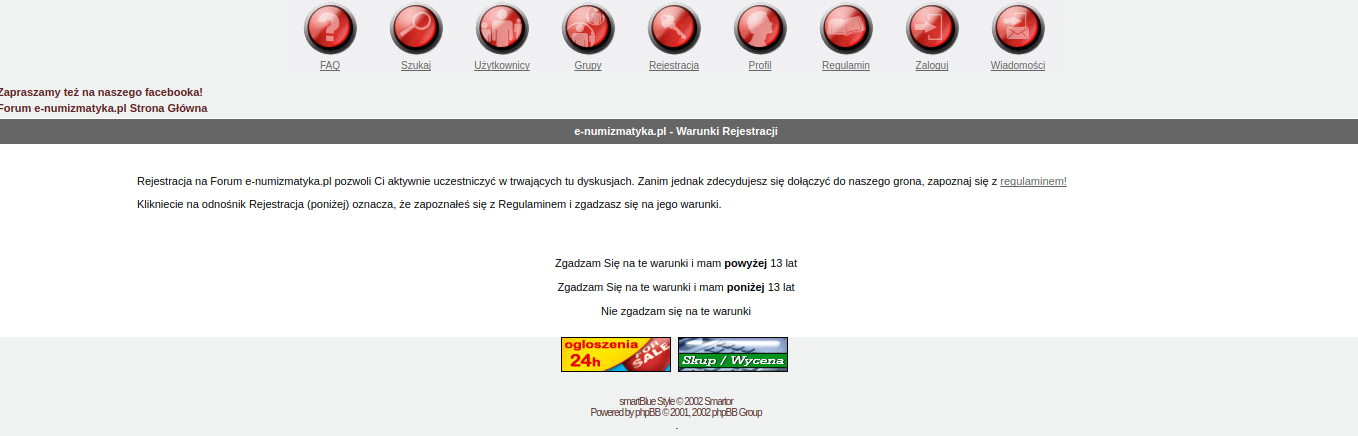
\includegraphics[width=\textwidth]{kck1}
\caption{Interfejs portalu e-numizmatyka.pl}
\end{center}
\begin{center}

\includegraphics[width=\textwidth]{kck2}
\caption{Formularz rejestracyjny}
\end{center}
Teraz nie dziwi nas fakt, że Andrzej nie znalazł tam nikogo ze swojej miejscowości. Te forum niczym nie zachęca nowych użytkowników do rejestracji sprawdziliśmy większość aktywnych użytkowników założyła konto pomiędzy 2003 a 2005 rokiem. Inne grupy które znaleźliśmy zajmowały się tylko i wyłącznie sprzedażą i wyceną.
\item[•]\textbf{Aleksander Pawletta}\newline
Pierwsze, co rzuciło się w oczy podczas przeglądania forum \url{http://pfmrc.eu} to brak poprawnego moderowania. W wątkach pojawia się wiele offtopów oraz dygresji polityczno-spiskowych. Tematom brak poprawnego otagowania. Co więcej, działanie wyszukiwarki pozostawia wiele do życzenia.
\begin{center}
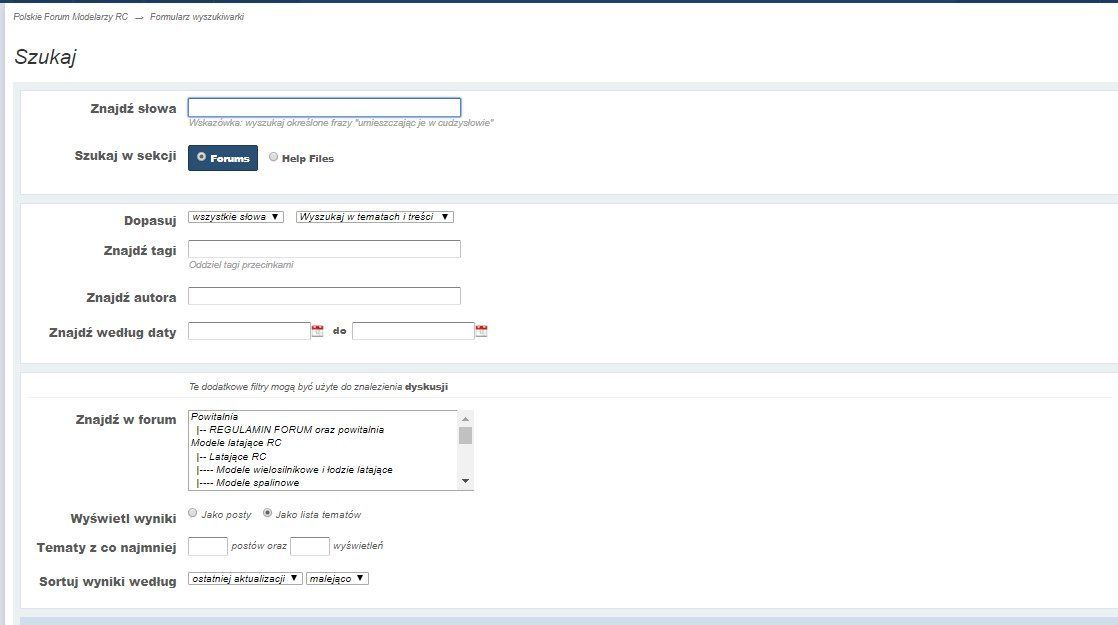
\includegraphics[width=\textwidth]{1}
\caption{wyszukiwarka na forum pfmrc.eu}
\end{center}
Jaki jest sens umieszczania szukanych fraz w cudzysłowiu?  Do tego rozmiar czcionki podpowiedzi prowadzi do jej niezauważenia, szczególnie gdy działamy w pośpiechu.
Ogółem szukana przez nas fraza (oczywiście nie stosując się do podpowiedzi dotyczącej jej wpisywania, niewidocznej bez wejścia do modułu wyszukiwarki)  pojawiła się dopiero w 12 wątku, a poprzedzające nie miały z nią nic wspólnego:
\begin{center}

\includegraphics[width=\textwidth]{2}
\end{center}
\begin{center}

\includegraphics[width=\textwidth]{3}
\end{center}
\newpage Po wyszukaniu frazy pole wyszukiwania zostaje wyczyszczone co jest dość irytujące jeżeli chcemy coś do niej dopisać.
Co więcej, jeżeli spróbujemy wyszukać kilka fraz w krótkim odstępie czasu naszym oczom ukazuje się:
\begin{center}
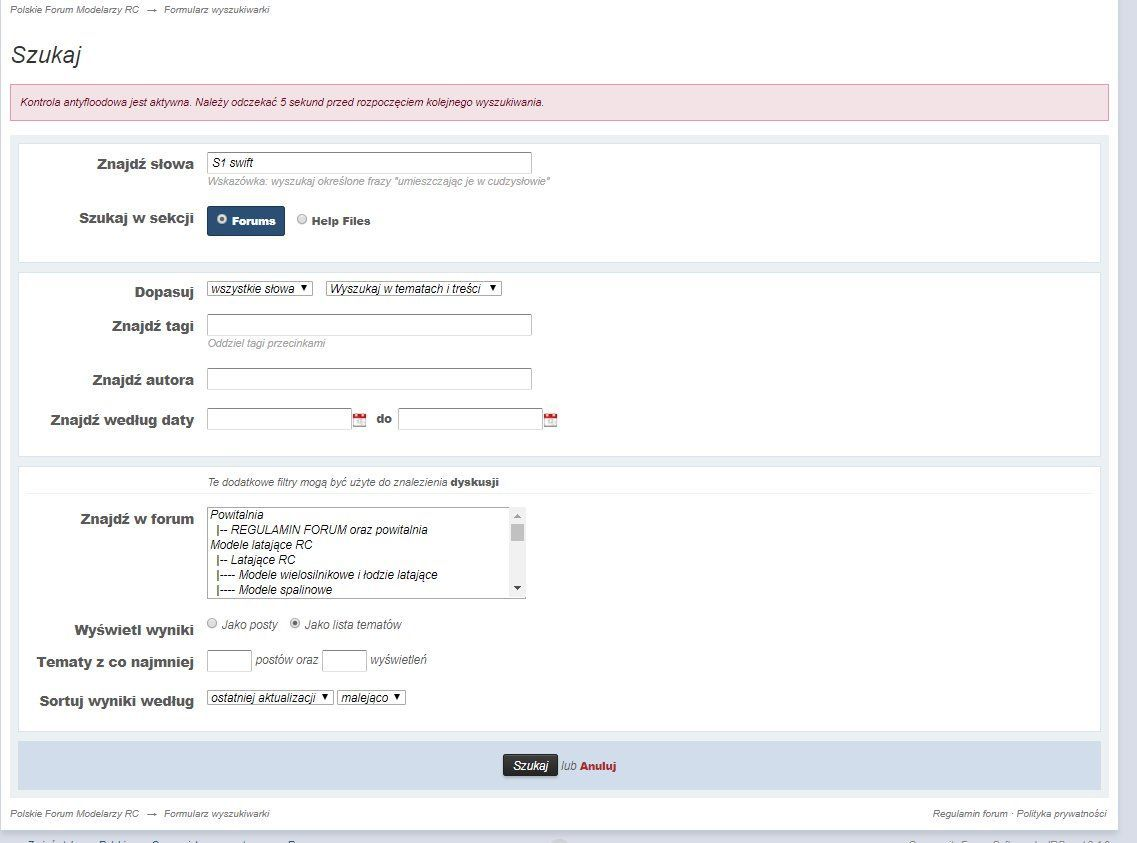
\includegraphics[width=\textwidth]{4}
\end{center}\newpage
Również wprowadzenie niedziałających właściwości przez twórców:
\begin{center}
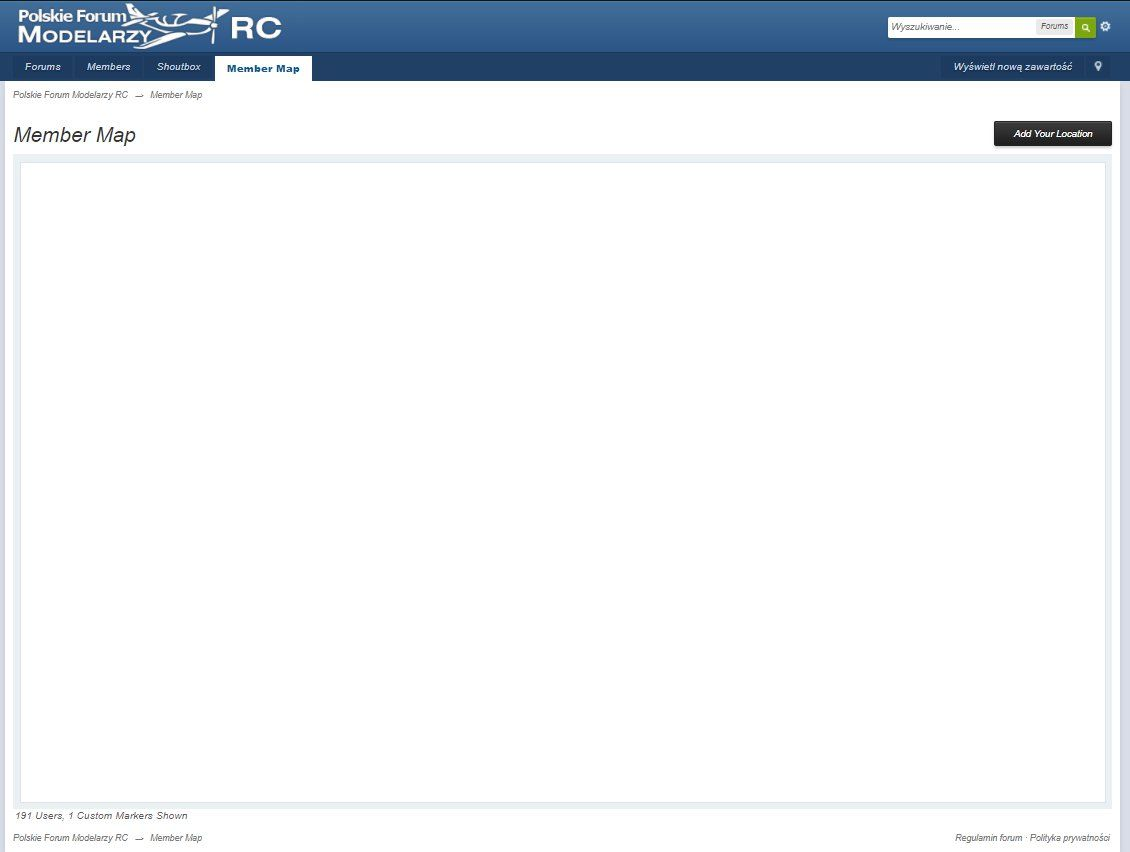
\includegraphics[width=\textwidth]{5}
\end{center}
W rozważanym przypadku prowadzi to do trwonienia czasu osób poszukujących pasjonatów w swojej okolicy.
\newpage 
\item[•]\textbf{Jakub Świst}\newline
Podobnie jak w przypadku Aleksandra, zauważyliśmy podobne błędy.
Rozpoczynając działanie na forum.airways.cz napotykamy problematyczne małe nieczytelne czcionki:
\begin{center}
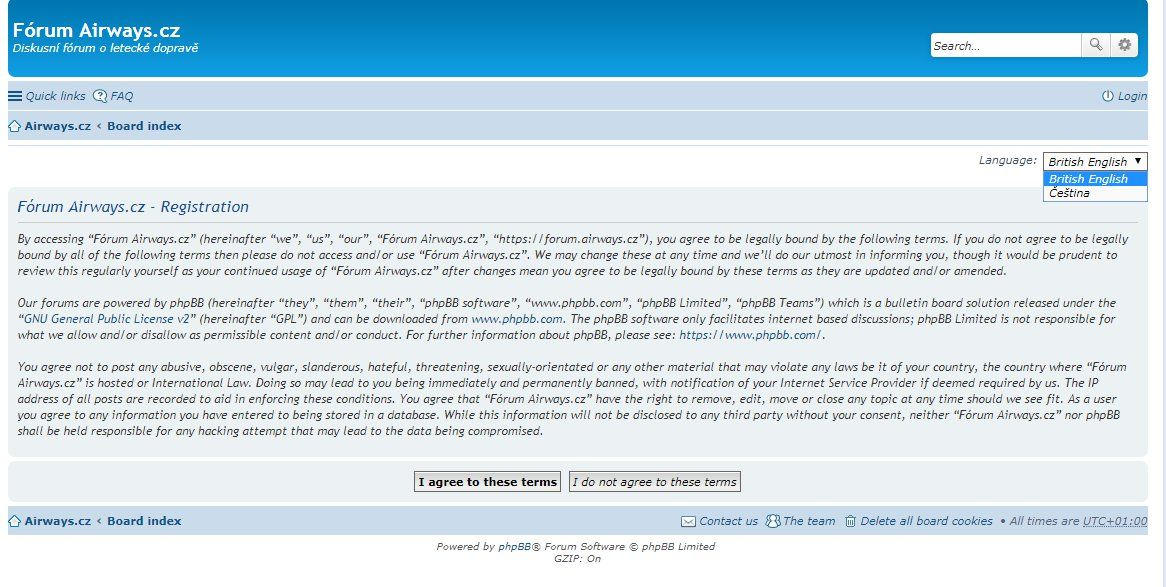
\includegraphics[width=\textwidth]{6}
\end{center}
Aczkolwiek miłym akcentem jest możliwość zmiany języka, co niestety nie dotyczy tekstu zawartego w osobnych wątkach oraz tematach. 
Co więcej, ich ilość znacznie utrudnia wyszukanie interesującej nas kwestii - poznania ludzi z okolicy, z którymi moglibyśmy dzielić się naszą pasją. Jednakże należy zwrócić uwagę na fakt, że nie projektowano tego forum w tym celu.Znalezienie osób chętnych do wzajemnego dzielenia się pasją na forum z mniejszą społecznością wydawałoby się znacznie prostsze. Jednakże forum aeroklubu Raná okazało się być wymarłe. Aktywność użytkowników pomiędzy 2007 a 2013 rokiem.
Małe, nieczytelne czcionki ograniczają znacznie starszych użytkowników tegoż forum. Również brak społeczności uniemożliwia osiągnięcie celu Jakuba.
\begin{center}
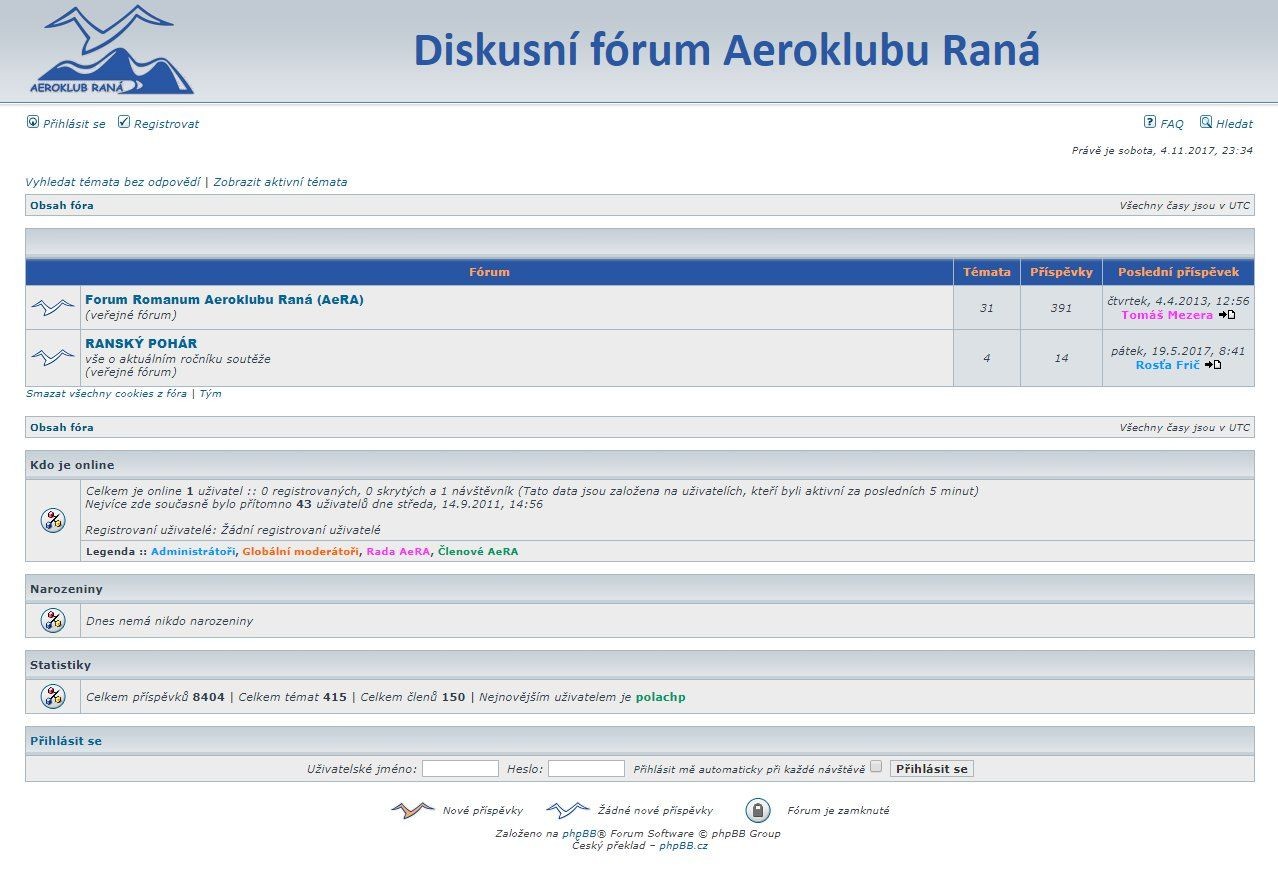
\includegraphics[width=\textwidth]{7}
\end{center}
\end{enumerate}
Ogółem brak platformy umożliwiającej zrealizowanie celu ankietowanym przysparza wiele kłopotów.
\newpage 
\section{Podsumowanie}
Na podstawie przeprowadzonych wywiadów można wyróżnić następujące potrzeby użytkowników  dostępnych dzisiaj interfejsów:
\begin{itemize}
\item[•]O wiele prościej i szybciej poznawać nowych ludzi na jednej platformie.
\item[•]Przydałby się system oceniania użytkowników. W przypadku takich hobby jak numizmatyka trudno jest zaufać nieznanym osobom i rozmawiać z nimi np. o swojej drogocennej kolekcji monet.
\item[•]Interfejs powinien być jak najbardziej prosty i intuicyjny, będą z niego korzystać ludzie w każdym wieku.
\item[•]Jako że nasza platforma zasięgiem ma obejmować europę środkowo- wschodnią, należałoby zaimplementować dobry międzyjęzykowy system tłumaczenia. 
\item[•]Przed wprowadzeniem, wszystkie możliwości platformy muszą zostać należycie przetestowane.
\item[•]Wartoby było zawierać w profilu użytkownika jakimi językami sprawnie się posługuje.
\item[•]Ciekawym dodatkiem mogłaby być możliwość poznawania czyiś zainteresowań poprzez na przykład losowe spotkania z innymi pasjonatami z naszej okolicy i nie tylko.
\end{itemize}
\end{document}